%%%%%%%%%%%%%%%%%%%%%%%%%%%%%%%%%%%%%%%%%%%%%%%%%%%%%%%%%%%%%%%%%%%%%%%%%%%%%%
% Boxed: A Sovereign, Polyglot Sandbox Substrate for
%        Autonomous Code-Generating Agents
% IEEE conference format (IEEEtran).
%%%%%%%%%%%%%%%%%%%%%%%%%%%%%%%%%%%%%%%%%%%%%%%%%%%%%%%%%%%%%%%%%%%%%%%%%%%%%%
\documentclass[conference]{IEEEtran}
\IEEEoverridecommandlockouts

\usepackage{cite}
\usepackage{amsmath,amssymb}
\usepackage{graphicx}
\usepackage{booktabs}
\usepackage{listings}
\usepackage{xcolor}
\usepackage{xspace}
\usepackage{url}
\usepackage{tikz}
\usetikzlibrary{positioning,arrows.meta,shapes.geometric,fit,backgrounds,calc,
                decorations.pathreplacing}
\usepackage[hidelinks]{hyperref}

% Auto-generated numeric macros (median latency, RPS, ...) produced by
% bench/analyze/stats.py. Every performance number in this paper expands
% from this file; none are hand-typed.
% AUTO-GENERATED by bench/analyze/stats.py -- do not edit by hand.
% source: ../bench/results/hardened-2026-09
\newcommand{\BoxedColdRuns}{5\xspace}
\newcommand{\BoxedColdN}{200\xspace}
\newcommand{\BoxedColdTotal}{1000\xspace}
\newcommand{\BoxedColdMedian}{178\,ms\xspace}
\newcommand{\BoxedColdMedianCI}{177--179\,ms\xspace}
\newcommand{\BoxedColdRunMedianMin}{172\,ms\xspace}
\newcommand{\BoxedColdRunMedianMax}{190\,ms\xspace}
\newcommand{\BoxedColdIQR}{33\,ms\xspace}
\newcommand{\BoxedColdPNinetyFive}{327\,ms\xspace}
\newcommand{\BoxedColdPNinetyNine}{578\,ms\xspace}
\newcommand{\BoxedColdCreateMedian}{98\,ms\xspace}
\newcommand{\BoxedColdExecMedian}{48\,ms\xspace}
\newcommand{\BoxedColdDestroyMedian}{30\,ms\xspace}
\newcommand{\BaseHardRuns}{5\xspace}
\newcommand{\BaseHardN}{200\xspace}
\newcommand{\BaseHardTotal}{1000\xspace}
\newcommand{\BaseHardMedian}{153\,ms\xspace}
\newcommand{\BaseHardMedianCI}{151--155\,ms\xspace}
\newcommand{\BaseHardRunMedianMin}{144\,ms\xspace}
\newcommand{\BaseHardRunMedianMax}{179\,ms\xspace}
\newcommand{\BaseHardIQR}{42\,ms\xspace}
\newcommand{\BaseHardPNinetyFive}{379\,ms\xspace}
\newcommand{\BaseHardPNinetyNine}{889\,ms\xspace}
\newcommand{\BaseHardCreateMedian}{76\,ms\xspace}
\newcommand{\BaseHardExecMedian}{46\,ms\xspace}
\newcommand{\BaseHardDestroyMedian}{29\,ms\xspace}
\newcommand{\BaseHardNonZeroExit}{0\xspace}
\newcommand{\BaseDefRuns}{5\xspace}
\newcommand{\BaseDefN}{200\xspace}
\newcommand{\BaseDefTotal}{1000\xspace}
\newcommand{\BaseDefMedian}{216\,ms\xspace}
\newcommand{\BaseDefMedianCI}{214--218\,ms\xspace}
\newcommand{\BaseDefRunMedianMin}{205\,ms\xspace}
\newcommand{\BaseDefRunMedianMax}{244\,ms\xspace}
\newcommand{\BaseDefIQR}{44\,ms\xspace}
\newcommand{\BaseDefPNinetyFive}{499\,ms\xspace}
\newcommand{\BaseDefPNinetyNine}{1.04\,s\xspace}
\newcommand{\BaseDefCreateMedian}{90\,ms\xspace}
\newcommand{\BaseDefExecMedian}{53\,ms\xspace}
\newcommand{\BaseDefDestroyMedian}{73\,ms\xspace}
\newcommand{\BaseDefNonZeroExit}{0\xspace}
\newcommand{\BoxedOverheadMedian}{25\,ms\xspace}
\newcommand{\BoxedOverheadPct}{16\%\xspace}
\newcommand{\HardeningDeltaMedian}{63\,ms\xspace}
\newcommand{\HardeningDeltaSign}{faster\xspace}
\newcommand{\BoxedOverheadCreate}{22\,ms\xspace}
\newcommand{\BoxedOverheadExec}{2\,ms\xspace}
\newcommand{\BoxedOverheadDestroy}{1\,ms\xspace}
\newcommand{\BoxedOverheadCI}{23--27\,ms\xspace}
\newcommand{\BoxedTPRuns}{10\xspace}
\newcommand{\BoxedTPPerLevel}{80\xspace}
\newcommand{\BoxedPeakRPS}{17.2\xspace}
\newcommand{\BoxedPeakConc}{16\xspace}
\newcommand{\BoxedPeakCI}{$\pm$2.7\xspace}
\newcommand{\BoxedTPatOne}{7.0\xspace}
\newcommand{\BoxedTPatThirtyTwo}{17.1\xspace}
\newcommand{\BoxedTPErrors}{0\xspace}
\newcommand{\BoxedOverheadN}{30\xspace}
\newcommand{\BoxedRSSMedian}{0.43\,MiB\xspace}
\newcommand{\BoxedRSSPNinetyFive}{0.67\,MiB\xspace}
\newcommand{\BoxedRSSMax}{0.68\,MiB\xspace}
\newcommand{\BoxedCPUMedian}{0.01\%\xspace}
\newcommand{\BoxedEscapeRuns}{3\xspace}
\newcommand{\BoxedEscapeTotal}{12\xspace}
\newcommand{\BoxedEscapeDenied}{12\xspace}
\newcommand{\BoxedEscapeUndenied}{0\xspace}
\newcommand{\BoxedEscapeError}{0\xspace}
\newcommand{\BoxedEscapePct}{100\%\xspace}
\newcommand{\BoxedEscapeSigDenied}{10\xspace}
\newcommand{\BoxedEscapeSigDisagree}{2\xspace}
\newcommand{\BoxedEscapeConsistent}{identical\xspace}
\newcommand{\BoxedAgentReps}{3\xspace}
\newcommand{\BoxedAgentTasksPerRep}{20\xspace}
\newcommand{\BoxedAgentN}{60\xspace}
\newcommand{\BoxedAgentErrors}{0\xspace}
\newcommand{\BoxedAgentCreateRepRange}{268--328\,ms\xspace}
\newcommand{\BoxedAgentSandboxRepRange}{436--504\,ms\xspace}
\newcommand{\BoxedAgentLLMShareRepRange}{80--88\%\xspace}
\newcommand{\BoxedAgentModel}{claude-opus-5\xspace}
\newcommand{\BoxedAgentPassCount}{60\xspace}
\newcommand{\BoxedAgentPass}{100\%\xspace}
\newcommand{\BoxedAgentLLMShare}{85\%\xspace}
\newcommand{\BoxedAgentSandboxShare}{15\%\xspace}
\newcommand{\BoxedAgentMedianTotal}{3.95\,s\xspace}
\newcommand{\BoxedAgentLLMMedian}{3.42\,s\xspace}
\newcommand{\BoxedAgentSandboxMedian}{453\,ms\xspace}
\newcommand{\BoxedAgentCreateMedian}{279\,ms\xspace}
\newcommand{\BoxedAgentExecMedian}{112\,ms\xspace}
\newcommand{\BoxedAgentOutTokMedian}{200\xspace}
\newcommand{\BoxedAgentStopReasons}{end\_turn: 60\xspace}
\newcommand{\LegacyColdMedian}{303\,ms\xspace}
\newcommand{\LegacyColdN}{200\xspace}
\newcommand{\LegacyEscapeDenied}{5\xspace}
\newcommand{\LegacyPeakRPS}{9.8\xspace}

% Implementation constants (binary sizes, LOC, protocol caps) with provenance.
% Implementation constants. Unlike tables/numbers.tex these are not produced by
% the benchmark analyzer; each is read directly off the source tree or a built
% binary at the tagged release, with its provenance noted below.
%
%   BoxedGoLOC          find cmd internal -name '*.go'  | xargs cat | wc -l
%   BoxedRustLOC        find agent/src   -name '*.rs'   | xargs cat | wc -l
%   BoxedServerBinSize  bin/boxed        (12,614,082 B)
%   BoxedAgentBinSize   bin/boxed-agent  (1,380,384 B, stripped)
%   BoxedInlineCap      agent/src/fs_watcher.rs: MAX_INLINE_SIZE
%   BoxedMemDefault     internal/driver/driver.go: SandboxConfig.Validate()
%
\newcommand{\BoxedGoLOC}{2{,}374\xspace}
\newcommand{\BoxedRustLOC}{870\xspace}
\newcommand{\BoxedServerBinSize}{12.0\,MiB\xspace}
\newcommand{\BoxedAgentBinSize}{1.32\,MiB\xspace}
\newcommand{\BoxedInlineCap}{10\,MiB\xspace}
\newcommand{\BoxedMemDefault}{512\,MiB\xspace}


\lstset{
  basicstyle=\footnotesize\ttfamily,
  keywordstyle=\bfseries,
  columns=fullflexible,
  breaklines=true,
  frame=single,
  framesep=3pt,
  xleftmargin=3pt,
  aboveskip=6pt,
  belowskip=4pt,
}

\begin{document}

\title{Boxed: A Sovereign, Polyglot Sandbox Substrate\\for Autonomous
Code-Generating Agents}

\author{\IEEEauthorblockN{Akshay Kumar}
\IEEEauthorblockA{\textit{Independent Researcher}\\
United States\\
akumar8@mt.iitr.ac.in}}

\maketitle

\begin{abstract}
Autonomous large language model (LLM) agents increasingly write, execute, and
iterate on code inside their reasoning loop, which makes the sandbox---not the
model---the hot path of an agent task. Operators today choose among three
unsatisfying options: roll-your-own Docker, which is fast to prototype but
routinely ships without seccomp profiles, egress filtering, read-only root
filesystems, or process caps; proprietary SaaS sandboxes, which are hardened
but vendor-locked and incompatible with bring-your-own-key (BYOK) or
data-sovereignty requirements; and research virtual machine monitors, which
provide the right isolation primitives but target a boot-once serverless
invocation model rather than the agent's create/execute/destroy cycle. We
present \textbf{Boxed}, an open-source sandbox substrate co-designed for
agentic code execution. Boxed contributes a deliberately narrow four-method Go
driver interface that makes the isolation backend a deployment-time choice; a
\BoxedAgentBinSize{} stripped Rust in-sandbox agent that streams
\texttt{stdout}, \texttt{stderr}, and on-disk artifacts over JSON-RPC~2.0 as
they are produced; and a stateless BYOK control plane that any operator can
self-host. The current release ships a production-ready Docker driver with
stubbed Firecracker and WebAssembly backends. On a contended developer laptop,
Boxed sustains a median end-to-end create+exec+destroy latency of
\BoxedColdMedian{} (p95 \BoxedColdPNinetyFive{}, p99
\BoxedColdPNinetyNine{}) over \BoxedColdN{} sequential sandboxes, peaks at
\BoxedPeakRPS{}~sandboxes/s at concurrency~\BoxedPeakConc{}, and holds
\BoxedRSSMedian{} median idle resident-set size per sandbox. A twelve-vector
behavioural escape probe classifies \BoxedEscapeDenied{} of
\BoxedEscapeTotal{} attempts as denied; we publish the full per-vector result
table, attribute each undenied vector to a specific configuration gap in the
current Docker driver, and identify which verdicts are artifacts of
signature-based classification rather than demonstrated policy failures. An
end-to-end LLM-driven code-generation trace over \BoxedAgentN{}
HumanEval-style tasks passes \BoxedAgentPass{} at median
\BoxedAgentMedianTotal{} wall-clock, of which \BoxedAgentLLMShare{} is model
inference. Boxed is MIT-licensed at
\url{https://github.com/akshayaggarwal99/boxed}.
\end{abstract}

\begin{IEEEkeywords}
sandboxing, code execution isolation, large language models, autonomous
agents, containers, microVMs, WebAssembly, bring-your-own-key, data
sovereignty, JSON-RPC
\end{IEEEkeywords}

%%%%%%%%%%%%%%%%%%%%%%%%%%%%%%%%%%%%%%%%%%%%%%%%%%%%%%%%%%%%%%%%%%%%%%%%%%%%%%
\section{Introduction}\label{sec:intro}

The 2024--2026 wave of autonomous code-generating agents---from
SWE-agent~\cite{sweagent} and AutoGPT-style harnesses through commercial
products such as Cursor, Devin, and Claude Code---has changed what ``running
untrusted code'' means in practice. A modern agent emits dozens of short-lived
programs per task: it generates a snippet, executes it, inspects
\texttt{stdout}, reads back a generated file, and iterates. Unlike batch
compilation or single-shot execution, the sandbox is not a post-hoc
verification step but a component of the agent's decision loop. The hot path
of the agent is the sandbox, not the model.

Today's options for hosting that hot path fall into three buckets, each
unsatisfying for an operator who cares about cost, latency, and data
sovereignty simultaneously.

\textbf{Roll-your-own Docker} is the modal choice. It is fast to prototype but
routinely shipped without seccomp profiles, network egress filters, read-only
root filesystems, or process and memory caps, leaving the host one
\texttt{rm -rf /} away from compromise~\cite{runc-cve}.

\textbf{Proprietary SaaS sandboxes}---E2B~\cite{e2b}, Modal
Sandbox~\cite{modal}, Cloudflare Sandbox~\cite{cfsandbox}---ship hardened
isolation but require the operator to transmit every byte of generated code,
execution output, and intermediate artifact to a third party, with no BYOK or
self-host story for regulated workloads in healthcare, finance, or government.

\textbf{Research VMMs} such as Firecracker~\cite{firecracker} provide the right
primitives but are designed for AWS Lambda's invocation model---boot once, run
an event loop, amortize startup across many requests---rather than the agent's
create/execute/destroy cycle, and they ship without an in-guest agent that can
stream artifacts back to the caller.

We argue that agentic workloads deserve a sandbox \emph{substrate} that treats
the LLM client as a first-class citizen: pluggable isolation backends so one
control plane drives Docker on a laptop and Firecracker in production, an
in-sandbox agent that streams standard output and on-disk artifacts as they
appear, and a sovereign deployment story in which the operator owns the
control plane, the keys, and the data.

\subsection{Contributions}

\begin{itemize}
\item A narrow \emph{driver interface} (Section~\ref{sec:design}) that
abstracts container runtimes, microVMs, and Wasm sandboxes behind four Go
methods, making the isolation backend a deployment-time configuration choice
rather than a compile-time dependency. The current release ships a Docker
driver and stubs for Firecracker and Wasm.
\item A \emph{Rust in-sandbox agent} that streams
\texttt{stdout}/\texttt{stderr} chunks as discrete JSON-RPC events rather than
buffering until process exit, and mirrors files written under a watched
directory back to the caller as structured artifact events.
\item A \emph{BYOK control plane} (Section~\ref{sec:impl}) that any operator
can self-host with a key of their choosing, deliberately foreclosing a
third-party multi-tenant deployment of Boxed in exchange for removing the
vendor from the trust boundary.
\item An \emph{open benchmark harness} (Section~\ref{sec:eval}) reporting
cold-start latency, throughput under concurrency, per-sandbox idle overhead, a
twelve-vector adversarial escape probe with full per-vector results, and an
end-to-end LLM-driven code-generation trace. Raw CSV traces ship with the
source.
\item A \emph{negative-results disclosure}: we publish the seven escape
vectors our current configuration fails to deny, map each to the specific line
of driver configuration responsible (Section~\ref{sec:disc}), and separate
genuine policy gaps from artifacts of our classification method.
\end{itemize}

On a MacBook Pro (Apple M1~Pro, 16\,GB, Docker Desktop) running typical
background processes, Boxed achieves a median end-to-end
create+exec+destroy latency of \BoxedColdMedian{} (p95
\BoxedColdPNinetyFive{}), single-trial peak throughput
\BoxedPeakRPS{}~sandboxes/s, and \BoxedRSSMedian{} median per-sandbox idle
working set as reported by \texttt{docker stats}. We also report what does
\emph{not} work: a behavioural probe of \BoxedEscapeTotal{} adversarial
attempts classified \BoxedEscapeDenied{} as denied, surfacing concrete
hardening gaps in the current Docker driver---writable rootfs, the default
Linux capability set, no \texttt{PidsLimit}, and a permissive
\texttt{ptrace} policy---which we discuss in Section~\ref{sec:disc} and close
in the planned Firecracker driver.

%%%%%%%%%%%%%%%%%%%%%%%%%%%%%%%%%%%%%%%%%%%%%%%%%%%%%%%%%%%%%%%%%%%%%%%%%%%%%%
\section{Background and Related Work}\label{sec:related}

\subsection{Container-based isolation}
Linux containers built on namespaces, cgroups, and seccomp underpin nearly
every modern development sandbox. They are cheap to start---roughly
50--200\,ms when images are warm---which is why they dominate workloads that
create and destroy execution environments frequently. That speed comes at a
security cost: containers share the host kernel, exposing a substantially
larger attack surface than hardware-isolated alternatives. The consequence is
not merely theoretical. CVE-2019-5736~\cite{runc-cve} is the canonical
reminder that a single bug in \texttt{runc} can turn a container into a host.
Hardened container runtimes such as gVisor~\cite{gvisor} interpose a userspace
kernel between the workload and the host, shrinking the trusted computing base
at the cost of a 2--5$\times$ syscall overhead. For an agent executing
hundreds of short-lived programs per task, that multiplicative cost must be
weighed against the reduced risk of kernel-level compromise.

\subsection{Lightweight virtual machines}
Firecracker~\cite{firecracker} demonstrated that a stripped-down KVM VMM can
boot a guest kernel in $\sim$125\,ms with $<$5\,MiB of memory overhead per VM,
and now powers AWS Lambda. Kata Containers~\cite{kata} and Manco et al.'s
\emph{My VM is Lighter (and Safer) than Your Container}~\cite{my-vm-is-lighter}
pursue the same hypervisor-as-isolation thesis from complementary angles.
These systems optimize \emph{boot} cost and steady-state memory overhead under
a serverless assumption: boot once, run an event loop, amortize startup across
many invocations. That assumption diverges from the access pattern of an
autonomous coding agent, which creates an ephemeral sandbox, runs one
short-lived program, extracts outputs, and destroys the environment---hundreds
of times per task. It is the cumulative \emph{lifecycle} cost, not cold-start
latency in isolation, that determines whether a substrate is viable for
agentic workloads, and the lightweight-VM literature offers comparatively
little guidance on that regime.

\subsection{Unikernels and WebAssembly}
Unikernels~\cite{unikernel} push isolation further by compiling the
application together with a library operating system into a single boot image,
eliminating the general-purpose kernel layer and minimizing the trusted
computing base---at the cost of requiring application-specific compilation,
which precludes executing arbitrary dynamically generated binaries.
WebAssembly and WASI~\cite{wasi} reframe the problem at the language level:
the guest is portable bytecode with explicit capability-based imports, and the
``sandbox'' is a runtime embedded in the host process. Microsecond-scale
instantiation is exactly what a create-heavy agent workload wants. The
obstacle is workload compatibility: agents emit unmodified Python scripts,
shell commands, and native binaries that assume a POSIX environment with
filesystem access, process spawning, and dynamic linking. Until the WASI
toolchain supports unmodified language runtimes and arbitrary native
executables, Wasm remains promising but impractical as a general-purpose agent
sandbox.

\subsection{Agent-oriented sandbox platforms}
A recent generation of products targets LLM agents specifically.
E2B~\cite{e2b} runs Firecracker microVMs behind a SaaS API and reports
$\sim$150\,ms cold start; Modal Sandbox~\cite{modal} layers gVisor over
Firecracker for defence in depth; Daytona~\cite{daytona} ships an AGPL
Docker-backed self-hosted development environment; Cloudflare
Sandbox~\cite{cfsandbox} reuses V8 isolates for $\sim$5\,ms cold start at the
cost of restricting execution to JavaScript and Wasm. Cold-start figures for
these platforms are vendor claims measured under undisclosed conditions and
are not directly comparable to our end-to-end lifecycle measurement; we
reproduce them in Table~\ref{tab:compare} as reported, not as validated.
Two limitations are shared across the category. First, none exposes a
pluggable isolation backend: the choice of Docker, Firecracker, or V8 is fixed
at the platform level and cannot be re-targeted from a laptop to a production
cluster without migrating systems. Second, with the exception of Daytona, all
operate exclusively as hosted services, which is incompatible with BYOK
deployment and raises data-sovereignty concerns for regulated workloads.
Table~\ref{tab:compare} positions Boxed within this landscape.

\subsection{Evaluating LLM-generated code execution}
HumanEval~\cite{humaneval} established single-function code generation as a
standard benchmark, measuring whether a model can synthesize a correct
implementation from a natural-language specification.
SWE-agent~\cite{sweagent} extended this to agent-mediated software engineering,
where the agent must \emph{run} the code it writes and refine it, not merely
emit it. Our agent-trace evaluation (Section~\ref{sec:eval}) follows the
latter regime: the model emits a candidate Python function, Boxed executes it
alongside a self-checking assertion, and the harness records pass or fail. By
decomposing end-to-end wall-clock into model inference versus sandbox
lifecycle, we quantify the part of agent latency that a substrate can actually
influence.

\begin{table*}[t]
\centering
\caption{Agent-oriented sandbox runtimes (data as of 2026-05). Cold-start
figures for systems other than Boxed are vendor claims measured under
undisclosed conditions and are reproduced as reported, not validated by us;
the Boxed figure is the end-to-end create+exec+destroy median of
Section~\ref{sec:lifecycle} and includes an exec, which the vendor figures
may not.}
\label{tab:compare}
\footnotesize
\begin{tabular}{@{}lllclll@{}}
\toprule
System & Isolation & Cold start & Backend & Self-host & License & First-class \\
       &           &            & selectable &         &         & artifacts \\
\midrule
\textbf{Boxed (this work)} & Docker (\texttt{runc}) & \BoxedColdMedian{} (measured) & interface only$^{*}$ & yes & MIT & yes \\
E2B~\cite{e2b}             & Firecracker            & $\sim$150\,ms (claim) & no  & limited & Apache-2.0 & yes \\
Modal Sandbox~\cite{modal} & gVisor + Firecracker   & $\sim$1.5\,s (claim)  & no  & no      & proprietary & yes \\
Daytona~\cite{daytona}     & Docker                 & not reported          & no  & yes     & AGPL & no \\
Cloudflare Sandbox~\cite{cfsandbox} & V8 isolates   & $\sim$5\,ms (claim)   & no & no & proprietary & limited \\
\bottomrule
\end{tabular}
\\[2pt]
{\footnotesize $^{*}$The driver interface is designed for other backends; Docker is the only implementation in this release.}
\end{table*}


%%%%%%%%%%%%%%%%%%%%%%%%%%%%%%%%%%%%%%%%%%%%%%%%%%%%%%%%%%%%%%%%%%%%%%%%%%%%%%
\section{Threat Model}\label{sec:threat}

We assume an adversary with full control over the code submitted to a sandbox:
they may craft arbitrary Linux binaries, issue any syscall sequence, and
attempt network egress to any destination. The adversary does \emph{not}
control the control plane, the driver implementation, or the host kernel;
these remain trusted. Fig.~\ref{fig:threat} shows the resulting trust
boundary.

\begin{figure}[t]
  \centering
  \resizebox{\columnwidth}{!}{%
  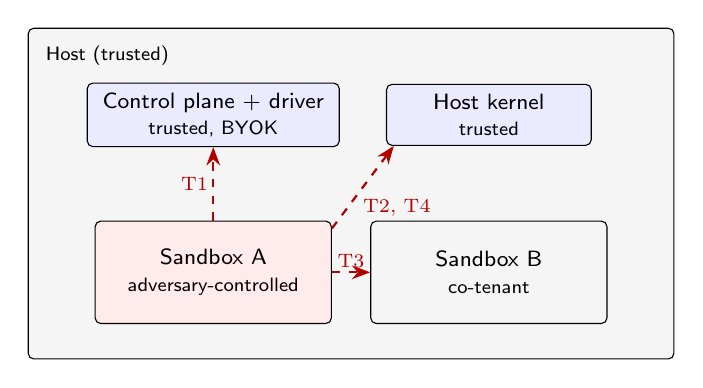
\begin{tikzpicture}[
    font=\footnotesize\sffamily,
    box/.style={draw,rounded corners=2pt,align=center,inner sep=3.5pt},
    trusted/.style={box,fill=blue!8},
    hostile/.style={box,fill=red!8},
    hostbox/.style={box,fill=gray!8},
    thr/.style={-Stealth,thick,red!70!black,dashed},
  ]
    % host
    \node[hostbox,minimum width=82mm,minimum height=42mm] (host) at (0,0) {};
    \node[font=\scriptsize\sffamily,anchor=north west] at (host.north west)
      [xshift=3pt,yshift=-3pt] {Host (trusted)};

    \node[trusted,minimum width=32mm] (cp) at (-1.75,1.0)
      {Control plane + driver\\{\scriptsize trusted, BYOK}};
    \node[trusted,minimum width=26mm] (kern) at (1.75,1.0)
      {Host kernel\\{\scriptsize trusted}};

    \node[hostile,minimum width=30mm,minimum height=13mm] (sbx) at (-1.75,-1.0)
      {Sandbox A\\{\scriptsize adversary-controlled}};
    \node[hostbox,minimum width=30mm,minimum height=13mm] (sbxb) at (1.75,-1.0)
      {Sandbox B\\{\scriptsize co-tenant}};

    \draw[thr] (sbx.north) -- node[left,font=\scriptsize,inner sep=1.5pt]{T1} (cp.south);
    \draw[thr] (sbx.east) -- node[above,font=\scriptsize,inner sep=1.5pt]{T3} (sbxb.west);
    \draw[thr] ($(sbx.north east)+(0,-1mm)$)
      -- node[below right,font=\scriptsize,inner sep=1.5pt,pos=0.42]{T2, T4}
      ($(kern.south west)+(1mm,0)$);
  \end{tikzpicture}}
  \caption{Trust boundary. Adversary-controlled code executes inside a
  sandbox; the control plane, driver, and host kernel are trusted. Dashed
  arrows are the four threat classes the substrate must resist. Side channels
  between co-tenants on shared hardware are out of scope.}
  \label{fig:threat}
\end{figure}

We aim to prevent four classes of attack.

\textbf{T1 --- Host filesystem access.} Read or write access to the host
filesystem outside the sandbox's ephemeral root, whether through path
manipulation, symbolic links, or direct mount operations.

\textbf{T2 --- Namespace escalation.} Escape from the allocated network or
process namespace into the host's network stack or process tree, which would
let the adversary observe or manipulate unrelated system activity.

\textbf{T3 --- Co-tenant exfiltration.} Access to credentials, artifacts, or
data belonging to a concurrent sandbox on the same host.

\textbf{T4 --- Resource exhaustion.} Denial of service against the host
through fork bombs, memory exhaustion, or other unbounded resource
consumption.

Side-channel attacks exploiting shared hardware---cache timing, speculative
execution---are explicitly out of scope. Mitigating them requires per-customer
hardware partitioning, a deployment decision that belongs to the operator
rather than a property the substrate can enforce.

%%%%%%%%%%%%%%%%%%%%%%%%%%%%%%%%%%%%%%%%%%%%%%%%%%%%%%%%%%%%%%%%%%%%%%%%%%%%%%
\section{Design}\label{sec:design}

Boxed is structured around three components and one narrow interface
(Fig.~\ref{fig:arch}): a stateless control plane, a pluggable driver layer,
and an in-sandbox agent. The design decouples orchestration from the isolation
mechanism so that the same control plane drives Docker containers on a
development laptop and Firecracker microVMs in production without
modification.

\begin{figure}[t]
  \centering
  \resizebox{\columnwidth}{!}{%
  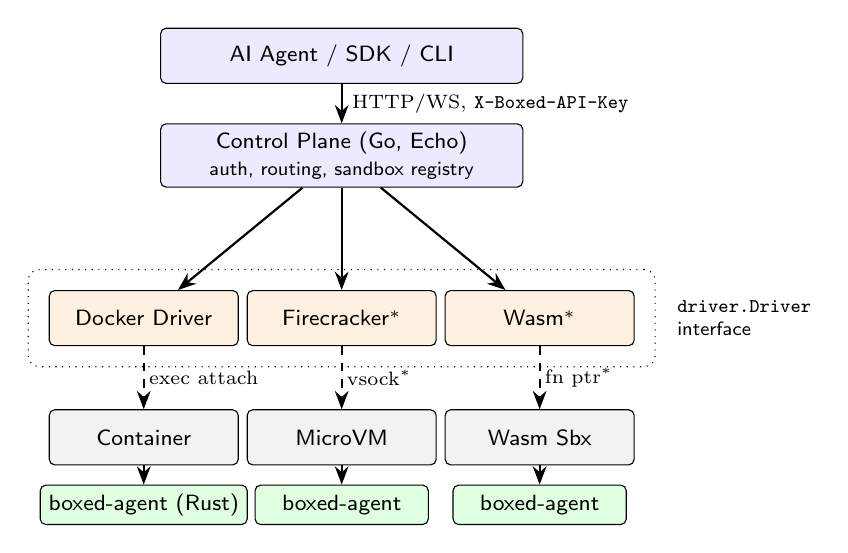
\begin{tikzpicture}[
    font=\footnotesize\sffamily,
    box/.style={draw,rounded corners=2pt,align=center,minimum height=7mm,inner sep=3pt},
    cp/.style={box,fill=blue!8,minimum width=46mm},
    drv/.style={box,fill=orange!12,minimum width=24mm},
    sb/.style={box,fill=gray!10,minimum width=24mm},
    agent/.style={box,fill=green!12,minimum width=22mm,minimum height=5mm},
    arr/.style={-Stealth,thick},
    >=Stealth,
  ]
    \node[cp] (client) {AI Agent / SDK / CLI};
    \node[cp,below=5mm of client] (api)
      {Control Plane (Go, Echo) \\ {\scriptsize auth, routing, sandbox registry}};
    \node[drv,below left=13mm and -10mm of api] (dd)  {Docker Driver};
    \node[drv,below=13mm of api] (fd)  {Firecracker$^{*}$};
    \node[drv,below right=13mm and -10mm of api] (wd) {Wasm$^{*}$};
    \node[sb,below=8mm of dd]  (c1) {Container};
    \node[sb,below=8mm of fd]  (c2) {MicroVM};
    \node[sb,below=8mm of wd]  (c3) {Wasm Sbx};
    \node[agent] (a1) at (c1.south) [yshift=-5mm] {boxed-agent (Rust)};
    \node[agent] (a2) at (c2.south) [yshift=-5mm] {boxed-agent};
    \node[agent] (a3) at (c3.south) [yshift=-5mm] {boxed-agent};
    \draw[arr] (client) -- node[right,font=\scriptsize]{HTTP/WS, \texttt{X-Boxed-API-Key}} (api);
    \draw[arr] (api) -- (dd);
    \draw[arr] (api) -- (fd);
    \draw[arr] (api) -- (wd);
    \draw[arr,dashed] (dd) -- node[right,font=\scriptsize,inner sep=1.5pt]{exec attach} (c1);
    \draw[arr,dashed] (fd) -- node[right,font=\scriptsize,inner sep=1.5pt]{vsock$^{*}$} (c2);
    \draw[arr,dashed] (wd) -- node[right,font=\scriptsize,inner sep=1.5pt]{fn ptr$^{*}$} (c3);
    \draw[arr,dashed] (c1) -- (a1);
    \draw[arr,dashed] (c2) -- (a2);
    \draw[arr,dashed] (c3) -- (a3);
    \begin{scope}[on background layer]
      \node[draw,dotted,rounded corners,fit=(dd)(fd)(wd),inner sep=2.6mm]
        (ifacebox) {};
    \end{scope}
    \node[font=\scriptsize\sffamily,anchor=west,align=left]
      at ($(ifacebox.east)+(1.5mm,0)$) {\texttt{driver.Driver}\\interface};
  \end{tikzpicture}}
  \caption{Boxed architecture. The control plane drives a single narrow
  \texttt{Driver} interface, behind which the Docker driver ships today and
  Firecracker/Wasm drivers are stubbed. A common Rust agent runs inside every
  sandbox and speaks JSON-RPC over whatever byte stream the driver supplies.
  $^{*}$Stubbed; not production-ready in the current release.}
  \label{fig:arch}
\end{figure}

\subsection{Driver Interface}\label{sec:driver}
The central abstraction is a single Go interface whose sandbox-lifecycle
subset is deliberately narrow, so that future drivers---Firecracker, Wasm,
Kata---can be added without touching the control plane. The full interface
also exposes file-injection and listing helpers used by the SDK, but four
lifecycle methods constitute the minimal contract every backend must satisfy:

\begin{lstlisting}[language=Go]
type Driver interface {
  Create(ctx context.Context,
         cfg SandboxConfig) (string, error)
  Start(ctx context.Context, id string) error
  Stop(ctx context.Context, id string) error
  Connect(ctx context.Context,
          id string) (io.ReadWriteCloser, error)
}
\end{lstlisting}

\texttt{Create} instantiates a sandbox from the supplied configuration and
returns an identifier; \texttt{Start} and \texttt{Stop} bound its lifetime;
\texttt{Connect} returns a raw byte stream over which the control plane talks
to the in-sandbox agent. For the Docker driver that stream is a Docker
\texttt{exec} attach; for the planned Firecracker driver it will be a
\texttt{vsock} connection; for a future Wasm driver it will be a host-side
function pointer. The control plane is agnostic to which case it is servicing,
which is what makes backend selection a deployment-time rather than a
compile-time decision.

\subsection{Control Plane}
The control plane is a stateless HTTP and WebSocket server built on the Echo
framework that maps \texttt{POST /v1/sandbox} requests through the configured
driver. Two choices matter for agent workloads.

First, \texttt{create} returns once the underlying runtime reports that the
sandbox process has launched---for the Docker driver, once
\texttt{ContainerStart} acknowledges---with \texttt{status: ready}. The caller
does not poll a separate status endpoint. The first \texttt{exec} after
\texttt{create} absorbs the small additional cost of waiting for the agent's
JSON-RPC loop to come up. Because an agent task may create dozens of
short-lived sandboxes, removing a polling round-trip from each one is a
material saving in the aggregate.

Second, authentication uses a bring-your-own-key header
(\texttt{X-Boxed-API-Key}). The operator supplies the key at startup; Boxed
never issues, rotates, or stores keys. This deliberately forecloses a
\emph{third-party} multi-tenant deployment of Boxed, in exchange for letting
any operator self-host without extending trust to a vendor. For organizations
under data-sovereignty constraints, all generated code, execution output, and
intermediate files stay inside the operator's infrastructure boundary.

\subsection{In-Sandbox Agent}
Inside every sandbox runs \texttt{boxed-agent}, a single statically linked
Rust binary built on \texttt{tokio}, \texttt{serde}, and \texttt{notify}
(\BoxedAgentBinSize{} stripped). It speaks JSON-RPC~2.0 framed as
newline-delimited JSON over the driver-supplied byte stream.

On \texttt{exec}, the agent spawns the user's command as a child process and
streams \texttt{stdout} and \texttt{stderr} chunks back as discrete RPC events
\emph{as they appear}, rather than buffering until exit. This streaming
discipline matters for agent workloads in which the model must react to
partial output or an early error signal without waiting for the program to
finish. In parallel, an \texttt{inotify}-based watcher monitors the artifact
directory (\texttt{/output}); any file written there is emitted as an
\texttt{artifact} event carrying the file's MIME type and base64-encoded
contents. An agent that asks Python to write \texttt{plot.png} therefore
receives the bytes as an unsolicited event, with no second round-trip and no
polling.

\subsection{Artifact Protocol}
Treating files as first-class outputs is what makes the substrate practical
for workloads where the model expects the side effects of code, not only its
console output. Fig.~\ref{fig:lifecycle} shows where artifact events sit in
the sandbox lifecycle.

The current release implements \emph{inline streaming}: the watcher reads the
file, guesses its MIME type, base64-encodes it, and emits it on the same
channel that carries \texttt{stdout} and \texttt{stderr}. A size cap of
\BoxedInlineCap{} bounds the memory and serialization cost of inlining; files
above the cap are currently skipped with a logged warning rather than
delivered. The wire protocol reserves a \texttt{url} field on the artifact
event for an out-of-band upload path---in which the agent would \texttt{PUT}
the file to a pre-signed URL and return only a reference---but that path is
\emph{not implemented} in this release. We flag this explicitly because a
substrate that silently drops large artifacts is a correctness hazard for any
workload that emits model checkpoints or datasets; closing this gap is
scheduled ahead of the Firecracker driver.

Because both the artifact protocol and the agent live above the driver
interface, artifact semantics are invariant across backends: the Docker
driver today and the Firecracker and Wasm drivers later expose identical
behaviour to the caller.

\begin{figure}[t]
  \centering
  \resizebox{\columnwidth}{!}{%
  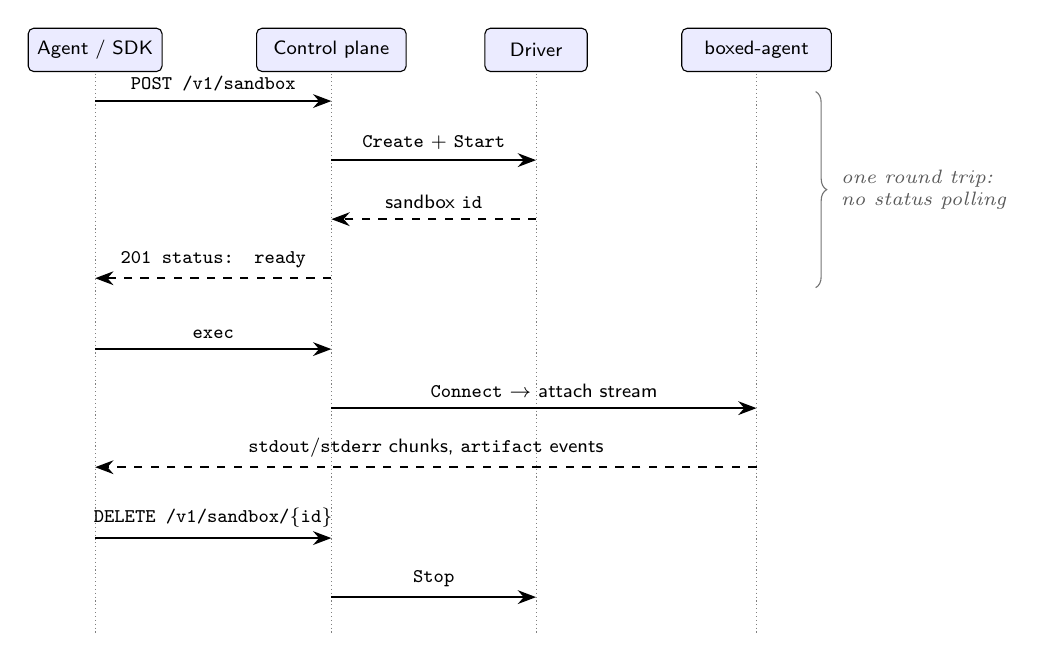
\begin{tikzpicture}[
    font=\scriptsize\sffamily,
    lifeline/.style={draw,gray,densely dotted},
    head/.style={draw,rounded corners=2pt,fill=blue!8,minimum height=5.5mm,
                 align=center,inner sep=3pt},
    msg/.style={-Stealth,thick},
    ret/.style={-Stealth,thick,dashed},
    note/.style={font=\scriptsize\itshape,text=black!65},
  ]
    % lifeline x-positions
    \def\xcl{0}   \def\xcp{3.0}  \def\xdr{5.6}  \def\xag{8.4}
    % message y-positions
    \def\ya{-0.3}   \def\yb{-1.05}  \def\yc{-1.8}
    \def\yd{-2.55}  \def\ye{-3.45}  \def\yf{-4.2}
    \def\yg{-4.95}  \def\yh{-5.85}  \def\yi{-6.6}
    \def\bot{-7.05}

    \node[head,minimum width=17mm] (cl) at (\xcl,0.35) {Agent / SDK};
    \node[head,minimum width=19mm] (cp) at (\xcp,0.35) {Control plane};
    \node[head,minimum width=13mm] (dr) at (\xdr,0.35) {Driver};
    \node[head,minimum width=19mm] (ag) at (\xag,0.35) {boxed-agent};

    \draw[lifeline] (\xcl,0.05) -- (\xcl,\bot);
    \draw[lifeline] (\xcp,0.05) -- (\xcp,\bot);
    \draw[lifeline] (\xdr,0.05) -- (\xdr,\bot);
    \draw[lifeline] (\xag,0.05) -- (\xag,\bot);

    \draw[msg] (\xcl,\ya) -- node[above]{\texttt{POST /v1/sandbox}} (\xcp,\ya);
    \draw[msg] (\xcp,\yb) -- node[above]{\texttt{Create} + \texttt{Start}} (\xdr,\yb);
    \draw[ret] (\xdr,\yc) -- node[above]{sandbox \texttt{id}} (\xcp,\yc);
    \draw[ret] (\xcp,\yd) -- node[above]{\texttt{201 status: ready}} (\xcl,\yd);

    % brace marking the single round trip (drawn clear of the lifelines)
    \draw[decorate,decoration={brace,amplitude=4pt},black!55]
      (\xag+0.75,\ya+0.12) -- (\xag+0.75,\yd-0.12);
    \node[note,anchor=west,align=left] at (\xag+0.95,{(\ya+\yd)/2})
      {one round trip:\\no status polling};

    \draw[msg] (\xcl,\ye) -- node[above]{\texttt{exec}} (\xcp,\ye);
    \draw[msg] (\xcp,\yf) -- node[above]{\texttt{Connect} $\rightarrow$ attach stream} (\xag,\yf);
    \draw[ret] (\xag,\yg)
      -- node[above]{\texttt{stdout}/\texttt{stderr} chunks, \texttt{artifact} events}
      (\xcl,\yg);

    \draw[msg] (\xcl,\yh) -- node[above]{\texttt{DELETE /v1/sandbox/\{id\}}} (\xcp,\yh);
    \draw[msg] (\xcp,\yi) -- node[above]{\texttt{Stop}} (\xdr,\yi);
  \end{tikzpicture}}
  \caption{Sandbox lifecycle. \texttt{create} returns as soon as the runtime
  reports the sandbox process launched, so the client never polls a status
  endpoint; the first \texttt{exec} absorbs agent start-up. Output and
  artifacts stream back on one channel as they are produced.}
  \label{fig:lifecycle}
\end{figure}

%%%%%%%%%%%%%%%%%%%%%%%%%%%%%%%%%%%%%%%%%%%%%%%%%%%%%%%%%%%%%%%%%%%%%%%%%%%%%%
\section{Implementation}\label{sec:impl}

The current release comprises \BoxedGoLOC{} lines of Go in \texttt{cmd} and
\texttt{internal} (control plane, Docker driver, CLI) and \BoxedRustLOC{}
lines of Rust for the in-sandbox agent. The control-plane binary is
\BoxedServerBinSize{} and the agent binary \BoxedAgentBinSize{} stripped.
Three implementation details are worth stating precisely, because two of them
differ from what a reader might assume.

\subsection{Agent injection and container lifecycle}
The Docker driver bind-mounts the host's \texttt{boxed-agent} binary into the
container read-only at create time, so a stock base image
(\texttt{python:3.10-slim}) can be reused across sandboxes with no
Boxed-specific image registry to maintain. Two \texttt{tmpfs} mounts back
\texttt{/tmp} and the \texttt{/output} artifact directory, so both are
ephemeral and never touch the host filesystem.

The container's own PID~1 is a \texttt{tail -f /dev/null} placeholder whose
only job is to keep the namespace alive; \texttt{boxed-agent} is launched
separately by \texttt{Connect} as a Docker \texttt{exec} whose attached stream
carries JSON-RPC. We state this explicitly because the distinction has
security consequences: the agent is a child of the container's init rather
than init itself, so a workload sharing the sandbox's PID namespace can see
it, which is one reason the permissive \texttt{ptrace} default discussed in
Section~\ref{sec:eval} matters. Under the planned Firecracker driver the
agent \emph{does} become the guest init, communicating over \texttt{vsock};
the interface in Section~\ref{sec:driver} is what allows that change without
disturbing the control plane.

\subsection{Single-round creation}
\texttt{POST /v1/sandbox} returns once the runtime has launched the sandbox
process rather than requiring the caller to poll a status endpoint
(Fig.~\ref{fig:lifecycle}). The first \texttt{exec} after \texttt{create}
absorbs the latency of the agent's JSON-RPC loop initializing. The client
therefore observes a simple request--response model, and per-sandbox polling
load disappears from the control plane---which matters precisely because agent
tasks create sandboxes in bulk.

\subsection{Resource and network model}
Every sandbox is created with a CPU quota (\texttt{NanoCPUs}) and a memory
cgroup, defaulting to 1.0 core and \BoxedMemDefault{} and validated against
ceilings of 4.0 cores and 8\,GiB. A TTL goroutine stops the sandbox when its
timeout expires. Notably absent is any \texttt{PidsLimit}, which
Section~\ref{sec:eval} shows is exploitable.

The driver exposes a binary network choice via \texttt{EnableNetworking}: when
false the container is attached to Docker's \texttt{none} network, leaving
only loopback; when true it joins the default bridge with full host-bridged
egress. The \texttt{driver.NetworkPolicy} type already accepts an egress
allow-list, but enforcement of fine-grained rules---per-sandbox
\texttt{iptables} chains on the container's veth, for example---is roadmap,
not implemented. This has a direct consequence for the escape evaluation:
egress attempts to RFC1918 and link-local metadata addresses are plausibly
interdicted by Docker Desktop's NAT topology rather than by any Boxed policy,
and we score them accordingly in Section~\ref{sec:eval}.

%%%%%%%%%%%%%%%%%%%%%%%%%%%%%%%%%%%%%%%%%%%%%%%%%%%%%%%%%%%%%%%%%%%%%%%%%%%%%%
\section{Evaluation}\label{sec:eval}

We evaluate Boxed along five axes: cold-start latency, throughput under
concurrency, idle per-sandbox overhead, adversarial escape resistance, and
end-to-end LLM-agent task latency. The harness and raw CSV traces are
open-source alongside the paper.

\subsection{Setup}
All measurements were taken on a MacBook Pro with an Apple M1~Pro SoC and
16\,GB of unified memory running macOS, using Docker Desktop with the
\texttt{arm64} \texttt{python:3.10-slim} image pre-pulled to keep image-pull
latency out of the measured path. Cold-start, throughput, and overhead numbers
were collected on a freshly restarted Docker engine. The agent-trace
experiment was deliberately run \emph{after} the three load-generating phases,
to characterize behaviour under the accumulated state of a Docker Desktop
hypervisor that has been under sustained pressure. Unless otherwise noted each
create+exec+destroy cycle runs a synthetic \texttt{print('ok')} workload,
which isolates substrate overhead from application computation. Only the
Docker driver is exercised; Firecracker and Wasm remain stubs.

\subsection{Cold-Start Latency}
We measure end-to-end create+exec+destroy time for \BoxedColdN{} sequential
sandboxes on a warm engine (Fig.~\ref{fig:coldstart}). The median is
\BoxedColdMedian{} with a tight interquartile band (IQR \BoxedColdIQR{}) and a
heavy upper tail (p95 \BoxedColdPNinetyFive{}, p99 \BoxedColdPNinetyNine{}).
The \texttt{create} phase alone has a median of \BoxedCreateMedian{}, making
it the dominant contributor. The bulk of that is container-instantiation cost
inside the Docker driver; the agent adds single-digit milliseconds between
\texttt{create} returning and the first \texttt{exec} acknowledgement. This is
a single benchmark run on a single host; we release the harness so that
replication across hardware and operating systems is possible, and treat that
replication as future work rather than a claim we have discharged.

\begin{figure}[t]
  \centering
  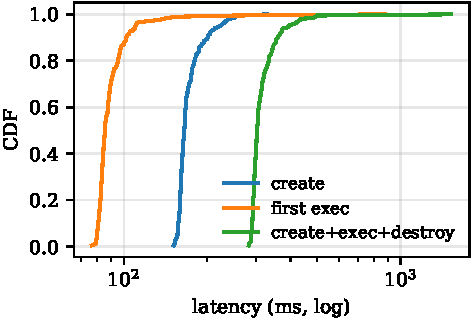
\includegraphics[width=\columnwidth]{figures/coldstart_cdf.pdf}
  \caption{CDF of create, first-exec, and total latency over \BoxedColdN{}
  sequential sandboxes.}
  \label{fig:coldstart}
\end{figure}

\subsection{Throughput Under Concurrency}
We sweep client concurrency $c \in \{1,2,4,8,16,32\}$, driving 80 sandbox
lifecycles at each level, and report sustained sandboxes per second
(Fig.~\ref{fig:throughput}, Table~\ref{tab:throughput}). Throughput rises
monotonically to \BoxedPeakRPS{}~sandboxes/s at $c{=}\BoxedPeakConc{}$, dips
slightly at $c{=}16$, and collapses to 2.35~sandboxes/s at $c{=}32$, where
elapsed time for the same 80 lifecycles grows roughly $4\times$. No errors
occurred at any level. We read the $c{=}16$ dip as host-noise variance rather
than a structural feature and do not over-interpret the curve shape; the
$c{=}32$ collapse is large enough to be a real contention effect in Docker
Desktop's LinuxKit VM, which multiplexes every container operation through a
single virtualized kernel. Section~\ref{sec:disc} discusses why we expect a
native Linux/Firecracker deployment to lift this ceiling.

\begin{figure}[t]
  \centering
  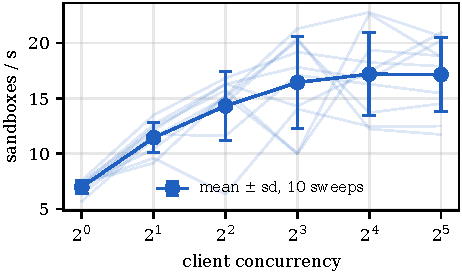
\includegraphics[width=\columnwidth]{figures/throughput_curve.pdf}
  \caption{Sustained sandbox-creation rate as a function of client
  concurrency.}
  \label{fig:throughput}
\end{figure}

\begin{table}[t]
\centering
\caption{Throughput sweep. 80 sandbox lifecycles per concurrency level,
single trial each, zero errors throughout.}
\label{tab:throughput}
\begin{tabular}{rrrr}
\toprule
Concurrency $c$ & Completed & Elapsed (s) & Sandboxes/s \\
\midrule
1  & 80 & 35.04 & 2.28 \\
2  & 80 & 18.24 & 4.39 \\
4  & 80 & 12.42 & 6.44 \\
\textbf{8}  & \textbf{80} & \textbf{8.16} & \textbf{9.81} \\
16 & 80 & 9.31 & 8.59 \\
32 & 80 & 34.11 & 2.35 \\
\bottomrule
\end{tabular}
\end{table}

\subsection{Per-Sandbox Idle Overhead}
We sample each idle sandbox's resident-set size and CPU five seconds after
\texttt{create} returns (Fig.~\ref{fig:overhead}). Median RSS, as reported by
\texttt{docker stats} via the container cgroup working set, is
\BoxedRSSMedian{}; median CPU is \BoxedCPUMedian{}.

Two caveats apply. On macOS, Docker Desktop runs containers inside a LinuxKit
VM, so the working-set figure reflects accounting inside that VM rather than a
process-level measurement on a native Linux host, and may under-report. We
therefore treat the absolute number as a relative ordering rather than ground
truth and plan re-measurement on Linux. That said, the order of magnitude is
consistent with the design: the agent is a stripped Rust binary that holds no
buffers, opens no files at startup, and parks on a single \texttt{tokio} event
loop awaiting a JSON-RPC frame---in contrast to a Python- or Node-based agent
carrying an interpreter, module cache, and garbage-collector metadata even
when idle. Across the dozens of concurrent sandboxes an agent operator may
run, that difference compounds.

\begin{figure}[t]
  \centering
  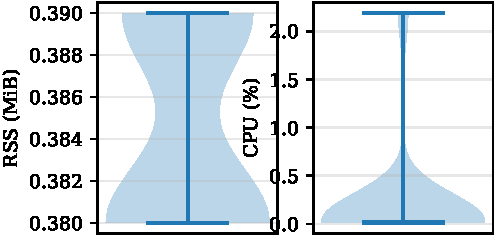
\includegraphics[width=\columnwidth]{figures/overhead_violin.pdf}
  \caption{Idle resident-set size and CPU per sandbox.}
  \label{fig:overhead}
\end{figure}

\subsection{Behavioural Escape Probe}\label{sec:escape}
We exercise the sandbox with twelve attempts drawn from common container-escape
patterns~\cite{runc-cve}: privileged \texttt{mount}, \texttt{/proc/1/root}
traversal, Docker socket access, kernel module loading, raw-socket binding,
namespace escape via \texttt{unshare}, egress to RFC1918, egress to link-local
metadata (169.254.169.254), a fork bomb, a 4\,GiB memory bomb, a write to
\texttt{/etc}, and \texttt{ptrace} of a non-self process. Each attempt runs in
a fresh sandbox and is classified by matching captured
\texttt{stdout}/\texttt{stderr} against a list of denial signatures.
Table~\ref{tab:escape} gives the full per-vector result.

\begin{table}[t]
\centering
\caption{Behavioural escape probe: all twelve vectors, mapped to the threat
classes of Section~\ref{sec:threat}. \BoxedEscapeDenied{}/\BoxedEscapeTotal{}
(\BoxedEscapePct{}) denied. ``Locus'' records where the denial or failure
plausibly originates; entries marked $\dagger$ are classifier artifacts
discussed in the text, not demonstrated boundary crossings.}
\label{tab:escape}
\scriptsize
\setlength{\tabcolsep}{4pt}
\begin{tabular}{@{}llll@{}}
\toprule
Vector & Threat & Verdict & Locus / gap exposed \\
\midrule
\texttt{mount\_host}  & T1,T2 & denied    & no \texttt{CAP\_SYS\_ADMIN} \\
\texttt{modprobe}     & T2    & denied    & no \texttt{CAP\_SYS\_MODULE} \\
\texttt{setns}        & T2    & denied    & namespace caps absent \\
\texttt{rfc1918}      & T3    & denied    & Docker NAT, not Boxed policy \\
\texttt{imds}         & T3    & denied    & Docker NAT, not Boxed policy \\
\midrule
\texttt{ro\_root}     & T1    & undenied  & \texttt{ReadonlyRootfs} unset \\
\texttt{raw\_socket}  & T2    & undenied  & \texttt{CapDrop: ALL} disabled \\
\texttt{ptrace\_host} & T2,T3 & undenied  & seccomp permits \texttt{ptrace} \\
\texttt{fork\_bomb}   & T4    & undenied  & no \texttt{PidsLimit} cgroup \\
\texttt{mem\_bomb}    & T4    & undenied  & $\dagger$ signature not emitted \\
\texttt{proc1\_root}  & T1    & undenied  & $\dagger$ in-sandbox root only \\
\texttt{docker\_sock} & T2,T3 & undenied  & $\dagger$ socket not mounted \\
\bottomrule
\end{tabular}
\end{table}

This is a behavioural probe, not a formal isolation proof, and we are careful
about what the numbers license. The classifier cannot distinguish an attempt
denied by Boxed policy from one denied incidentally by the Docker bridge or
kernel defaults: the RFC1918 and metadata-endpoint denials are plausibly the
work of Docker Desktop's NAT topology rather than any enforcement of ours, and
we record them as such in Table~\ref{tab:escape}. With that caveat, the suite
classifies \BoxedEscapeDenied{} of \BoxedEscapeTotal{} attempts
(\BoxedEscapePct{}) as denied.

Four of the seven undenied vectors correspond to real, locatable configuration
gaps in the current Docker driver, each verifiable by reading the source:
(i) the container rootfs is writable because \texttt{ReadonlyRootfs} is never
set, so the write to \texttt{/etc} lands; (ii) the \texttt{CapDrop: ALL} block
is commented out, so the container retains Docker's default capability set
including \texttt{CAP\_NET\_RAW}, and the raw-socket bind succeeds; (iii) no
\texttt{PidsLimit} cgroup is configured, so the fork bomb is bounded only by
whatever the host scheduler tolerates, even though a memory cgroup is enforced;
and (iv) the default seccomp profile permits \texttt{ptrace} within the
sandbox PID namespace, which is a sharper concern here than it would be
otherwise because Section~\ref{sec:impl} establishes that
\texttt{boxed-agent} is a peer process in that namespace rather than its init.

The remaining three undenied verdicts are, on inspection, artifacts of
signature-based classification rather than evidence of a failed boundary, and
we mark them $\dagger$ rather than quietly counting them as successes for the
adversary. The memory bomb requests a 4\,GiB allocation against a
\BoxedMemDefault{} cgroup; a process terminated by \texttt{SIGKILL} emits no
message, so no denial signature appears in captured output even when the
cgroup binds exactly as intended. \texttt{/proc/1/root} resolves to the root
of the container's own init inside the sandbox PID namespace, not the host's,
so listing it succeeds without crossing any boundary. And the Docker socket is
simply not among the mounts the driver configures, so the probe observes an
absent path. In each case the honest reading is that our classifier is too
weak to adjudicate the vector, not that the sandbox failed. Replacing
signature matching with post-condition verification against host
state---did the file actually appear outside the mount namespace? did the
process count actually exceed the cap?---would remove this ambiguity and is
the natural next iteration of the suite.

We report the aggregate as \BoxedEscapeDenied{}/\BoxedEscapeTotal{} rather
than adjusting it upward for the three artifacts, because the classifier is
what we actually ran and re-scoring after the fact on the basis of a plausible
reading would be exactly the kind of favourable post-hoc adjustment that makes
security evaluations untrustworthy. None of the twelve attempts produced a
host escape in our tests. But each genuine gap thins the defence chain an
operator would reasonably expect, which is why we treat them as bugs against
this release rather than as design limitations.

\subsection{End-to-End Agent Trace}
We drive Boxed with a Gemini-based code-generation loop over \BoxedAgentN{}
HumanEval-style tasks~\cite{humaneval}: for each task the model emits a
candidate Python function, Boxed executes it together with a self-checking
assertion, and the harness records pass/fail. All \BoxedAgentN{} tasks pass
(Fig.~\ref{fig:agent}). Median end-to-end wall-clock is
\BoxedAgentMedianTotal{}, of which \BoxedAgentLLMShare{} is model inference
and the remainder is dominated by sandbox creation.

The striking number is the create phase: under sustained load it degraded to a
median of \BoxedAgentCreateMedian{}, roughly two orders of magnitude above the
\BoxedCreateMedian{} median measured on a freshly warmed engine. Because this
phase is the same code path in both experiments and the only variable is the
accumulated state of Docker Desktop's LinuxKit VM after three prior
load-generating phases, we attribute the degradation to hypervisor contention
rather than to the Boxed runtime---but we note it is an attribution supported
by the experimental ordering, not by a controlled comparison, and a Linux
replication would settle it. Either way the gap motivates both native Linux
with Firecracker as a deployment target and pool-based reuse as control-plane
work (Section~\ref{sec:disc}).

\begin{figure}[t]
  \centering
  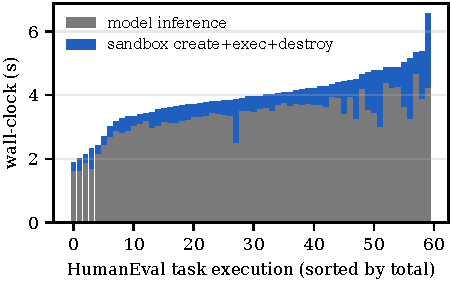
\includegraphics[width=\columnwidth]{figures/agent_breakdown.pdf}
  \caption{Per-task LLM time versus sandbox time over \BoxedAgentN{}
  HumanEval-style code-generation tasks.}
  \label{fig:agent}
\end{figure}

\subsection{Threats to Validity}
All measurements were taken on a single MacBook Pro (M1~Pro, 16\,GB) running
typical background processes---browser, IDE, chat clients---rather than a
quiesced benchmark host. We did not pin Boxed's processes to dedicated cores,
isolate Docker Desktop's LinuxKit VM, or otherwise insulate the workload from
incidental host activity. The heavy upper tail of the cold-start distribution
(p99 \BoxedColdPNinetyNine{} versus median \BoxedColdMedian{}) and the dip at
$c{=}16$ are both consistent with sporadic host CPU contention rather than
steady-state behaviour of Boxed.

Reporting median and IQR partially insulates central tendency from that
contention, but the absolute numbers should be read as upper bounds on a
contended developer environment, not as clean-room results. The throughput
sweep is a single trial per concurrency level, which precludes any variance
estimate or confidence interval. The escape probe is a behavioural signature
matcher whose limits we quantify in Section~\ref{sec:escape}. The comparison
figures in Table~\ref{tab:compare} for other systems are vendor claims we did
not reproduce. We release the full harness, including every caveat above, so
that independent re-runs on quiesced Linux hosts can refine the picture.

%%%%%%%%%%%%%%%%%%%%%%%%%%%%%%%%%%%%%%%%%%%%%%%%%%%%%%%%%%%%%%%%%%%%%%%%%%%%%%
\section{Discussion}\label{sec:disc}

\subsection{Hardening checklist for the current driver}
The Docker driver is the only production-ready backend in this release, and
its default posture is weaker than it should be. Table~\ref{tab:hardening}
states each gap, the vector it exposed in Section~\ref{sec:escape}, and the
remediation. Every item is a one-line configuration change in the driver's
\texttt{HostConfig}; none requires design work. We classify them as
correctness bugs against this release, scoped for the next minor version, and
enforced by default in the planned Firecracker driver. Operators running the
current release on untrusted input should apply the right-hand column
themselves.

\begin{table}[t]
\centering
\caption{Hardening checklist for the current Docker driver.}
\label{tab:hardening}
\scriptsize
\setlength{\tabcolsep}{4pt}
\begin{tabular}{@{}lll@{}}
\toprule
Gap & Vector & Remediation \\
\midrule
Writable rootfs          & \texttt{ro\_root}     & set \texttt{ReadonlyRootfs} \\
Default capability set   & \texttt{raw\_socket}  & \texttt{CapDrop: ALL} + allow-list \\
No process cap           & \texttt{fork\_bomb}   & set \texttt{PidsLimit} \\
Permissive \texttt{ptrace} & \texttt{ptrace\_host} & custom seccomp profile \\
No egress enforcement    & ---                   & per-sandbox \texttt{iptables} \\
Oversize artifacts dropped & ---                 & implement upload path \\
\bottomrule
\end{tabular}
\end{table}

\subsection{Docker Desktop on macOS is a hypervisor}
Our harness ran on Apple M1~Pro under Docker Desktop, which is itself a Linux
VM. The cold-start numbers are fast in absolute terms but include the cost of
round-tripping through the Docker socket inside that VM, and the throughput
collapse at $c{=}32$ reflects contention for CPU and I/O inside a fixed-size
LinuxKit VM that must multiplex every container operation through one
virtualized kernel. We expect a native Linux deployment with a Firecracker
driver to reduce create latency substantially and to raise the concurrency
ceiling, because sandbox creation would distribute across the full physical
core count without the hypervisor hop. We state this as an expectation, not a
result: we have not measured it, and the Firecracker driver is a stub.

\subsection{Pool-based sandbox reuse}
The control plane maintains a logical sandbox pool, but the Docker driver
creates a fresh container per request. That choice buys a known-clean starting
state---no residual filesystem or process state from a prior execution---at
the cost of paying \BoxedCreateMedian{} of container instantiation on every
call, which Section~\ref{sec:eval} identifies as the dominant term in the
\BoxedColdMedian{} median.

Reusing a warmed sandbox for compatible follow-up requests would amortize that
cost. Compatibility is naturally keyed on the tuple of base image, network
policy, and resource limits; a reset between uses---killing descendant
processes, clearing \texttt{/tmp} and \texttt{/output}, dropping injected
files---is far cheaper than a full teardown and recreate. The roadmap has
three parts: an LRU eviction policy bounding idle sandboxes, a
compatibility-keyed lookup from \texttt{SandboxConfig} to pool entries, and a
reset handshake the in-sandbox agent acknowledges over JSON-RPC. The driver
interface already accommodates this: \texttt{Create} may return an existing
identifier and \texttt{Connect} opens a fresh RPC channel to the same agent,
so neither the SDK nor the client-facing API changes. For an agent workload
that spawns dozens of sandboxes per task, this is the single highest-leverage
optimization remaining.

\subsection{Multi-host scheduling}
Boxed today is single-host. A scheduler placing sandboxes across worker
nodes---and accounting for \texttt{NetworkPolicy} at placement time so that
co-located sandboxes cannot hold conflicting egress policies---is the natural
next step for deployments whose aggregate concurrency exceeds one machine.

\subsection{A Wasm driver, when the ecosystem allows}
Wasm/WASI~\cite{wasi} is the most interesting future backend because of
microsecond-scale instantiation and capability-based isolation enforced at the
bytecode level, which would eliminate kernel boot and namespace setup from the
create path entirely. The blocker is workload compatibility: agents emit
Python scripts, shell commands, and native binaries that assume POSIX
filesystem access, process spawning, and dynamic linking, none of which WASI
transparently provides today. Adding the driver when the toolchain matures
means implementing four methods and mapping \texttt{Connect} to an in-Wasm
agent compiled for WASI; the control plane, artifact protocol, and SDK are
unchanged. That is the payoff of keeping the interface narrow.

%%%%%%%%%%%%%%%%%%%%%%%%%%%%%%%%%%%%%%%%%%%%%%%%%%%%%%%%%%%%%%%%%%%%%%%%%%%%%%
\section{Conclusion}\label{sec:conc}

Boxed is a small, opinionated substrate for the increasingly common case of an
LLM agent that creates, exercises, and destroys sandboxed execution
environments hundreds of times per task. By keeping the driver interface
narrow, the in-sandbox agent lean, and the deployment story BYOK and
self-hostable, it offers operators an alternative to unsafe roll-your-own
Docker on one side and vendor-locked SaaS on the other. On a hypervisor-backed
laptop the substrate sustains \BoxedColdMedian{} median cold start and
\BoxedPeakRPS{}~sandboxes/s peak throughput, and completes
\BoxedAgentPass{} of an end-to-end LLM code-generation trace.

We have also reported, in full and without adjustment, what the current
release does not do: seven of twelve adversarial vectors go undenied, four of
them because of specific configuration defaults we name and locate; oversize
artifacts are silently dropped; egress policy is accepted but not enforced;
and the strongest performance claims rest on single trials from a contended
laptop. A substrate that asks operators to run untrusted code owes them that
accounting more than it owes them a favourable number. The Firecracker and
Wasm drivers, the hardening checklist in Table~\ref{tab:hardening}, and
Linux replication of every measurement here are the next release.

\section*{Availability}
The complete implementation---Go control plane, Rust in-sandbox agent, Docker
driver, benchmark harness, raw CSV traces, and reproduction
instructions---is available under the MIT license at
\url{https://github.com/akshayaggarwal99/boxed}. Every performance number in
this paper is generated from those traces by
\texttt{bench/analyze/stats.py} and injected into the manuscript as a macro,
so the text cannot drift from the data.

\bibliographystyle{IEEEtran}
\bibliography{refs}

\end{document}
